\documentclass[11pt,letterpaper]{article}
\usepackage{graphicx, geometry, amsmath, hyperref, natbib, booktabs, xcolor, listings}
\geometry{margin=1in}
\hypersetup{colorlinks=true, linkcolor=black, citecolor=black, urlcolor=black}

\lstset{
  basicstyle=\small\ttfamily,
  columns=fullflexible,
  frame=single,
  breaklines=true,
  postbreak=\mbox{\textcolor{red}{$\hookrightarrow$}\space},
}

\title{Energy-Guided MCMC Sampling for Neuro-Symbolic Text-to-FOL Translation with Reversible Semantic Accommodation}
\author{Anonymous}
\date{}

\begin{document}

\maketitle

\begin{abstract}
Neuro-symbolic approaches to text-to-first-order-logic (FOL) translation face two critical limitations: they generate deterministic translations that cannot recover from early errors, and they handle ambiguity through brittle symbolic matching or black-box neural probabilities, leading to hallucinations. We introduce a novel neuro-symbolic architecture that addresses these limitations through three key innovations: (1) Markov Chain Monte Carlo (MCMC) sampling over complete Datalog programs guided by a composite energy function combining semantic fidelity, ontological consistency via ConceptNet, and logical coherence; (2) reversible semantic accommodation with provenance tracking and confidence-gated insertion to minimize hallucination; and (3) human-auditable trace-graphs showing which facts are text-derived versus system-accommodated. We validate the core assumption that LLMs can generate diverse, valid FOL fragments through a pilot experiment on RuleTaker data, achieving 100\% valid fragment rate with multi-stage syntax validation. While semantic diversity with mock LLM responses was limited (mean pairwise cosine distance = 0.008), the validation pipeline supports temperature-scaled diverse generation. Our mathematical specification of the composite energy function E = w1*E\_text + w2*E\_onto + w3*E\_cohere provides a foundation for energy-guided sampling of logic programs. The proposed architecture bridges statistical mechanics (MCMC sampling), linguistics (semantic accommodation), and database theory (provenance tracking) in a unified neuro-symbolic framework.
\end{abstract}

\section{Introduction}

Translating natural language text into formal logical representations is a foundational challenge in artificial intelligence, with applications spanning question answering, knowledge base construction, and automated reasoning \cite{Clark2020}. The dominant approaches to this task fall into two paradigms: purely neural methods that use large language models (LLMs) to generate logical forms directly, and neuro-symbolic methods that combine neural translation with symbolic reasoning engines \cite{Pan2023, Rocktaschel2017}.

Despite recent progress, existing approaches suffer from two critical limitations. First, they generate a single deterministic FOL translation that cannot recover from early translation errors. If the initial translation is flawed, the entire reasoning pipeline fails. Second, they handle ambiguity through either brittle symbolic matching (e.g., Prolog-based parsers) or black-box neural probabilities (e.g., LLM token probabilities), both of which lead to hallucinations or reasoning failures \cite{Ji2023}.

Consider the task of reasoning over a text: ``Alice is a cat. Bob is a dog. Cats like mice. Dogs like bones. Alice likes mice.'' A deterministic translation might incorrectly represent ``Alice likes mice'' as a general rule rather than a specific fact, leading to incorrect generalizations. Moreover, if the system encounters missing information (e.g., ``Does Alice like bones?''), it cannot gracefully accommodate the missing fact without risking hallucination.

To address these limitations, we draw inspiration from three distinct fields:

\begin{enumerate}
  \item \textbf{Statistical Mechanics}: Markov Chain Monte Carlo (MCMC) methods and energy-based models suggest that optimal logic translations can be found by sampling from an energy landscape rather than deterministic optimization \cite{LeCun2006}. MCMC provides a computationally feasible approximation to full Boltzmann sampling over combinatorial fragment spaces.
  
  \item \textbf{Linguistics}: Semantic accommodation (Lewis, 1979) describes how humans handle missing information by inserting plausible assumptions \cite{Lewis1979}. Making accommodation reversible (via provenance-tracked LIFO stack) and confidence-gated (LLM self-evaluation >0.8) prevents error accumulation.
  
  \item \textbf{Database Theory}: Provenance tracking (recording where each fact originated) and Datalog (a decidable logic fragment) enable human-auditable traces and tractable contradiction detection \cite{Ceri1989}.
\end{enumerate}

\begin{figure*}[!t]
  \centering
  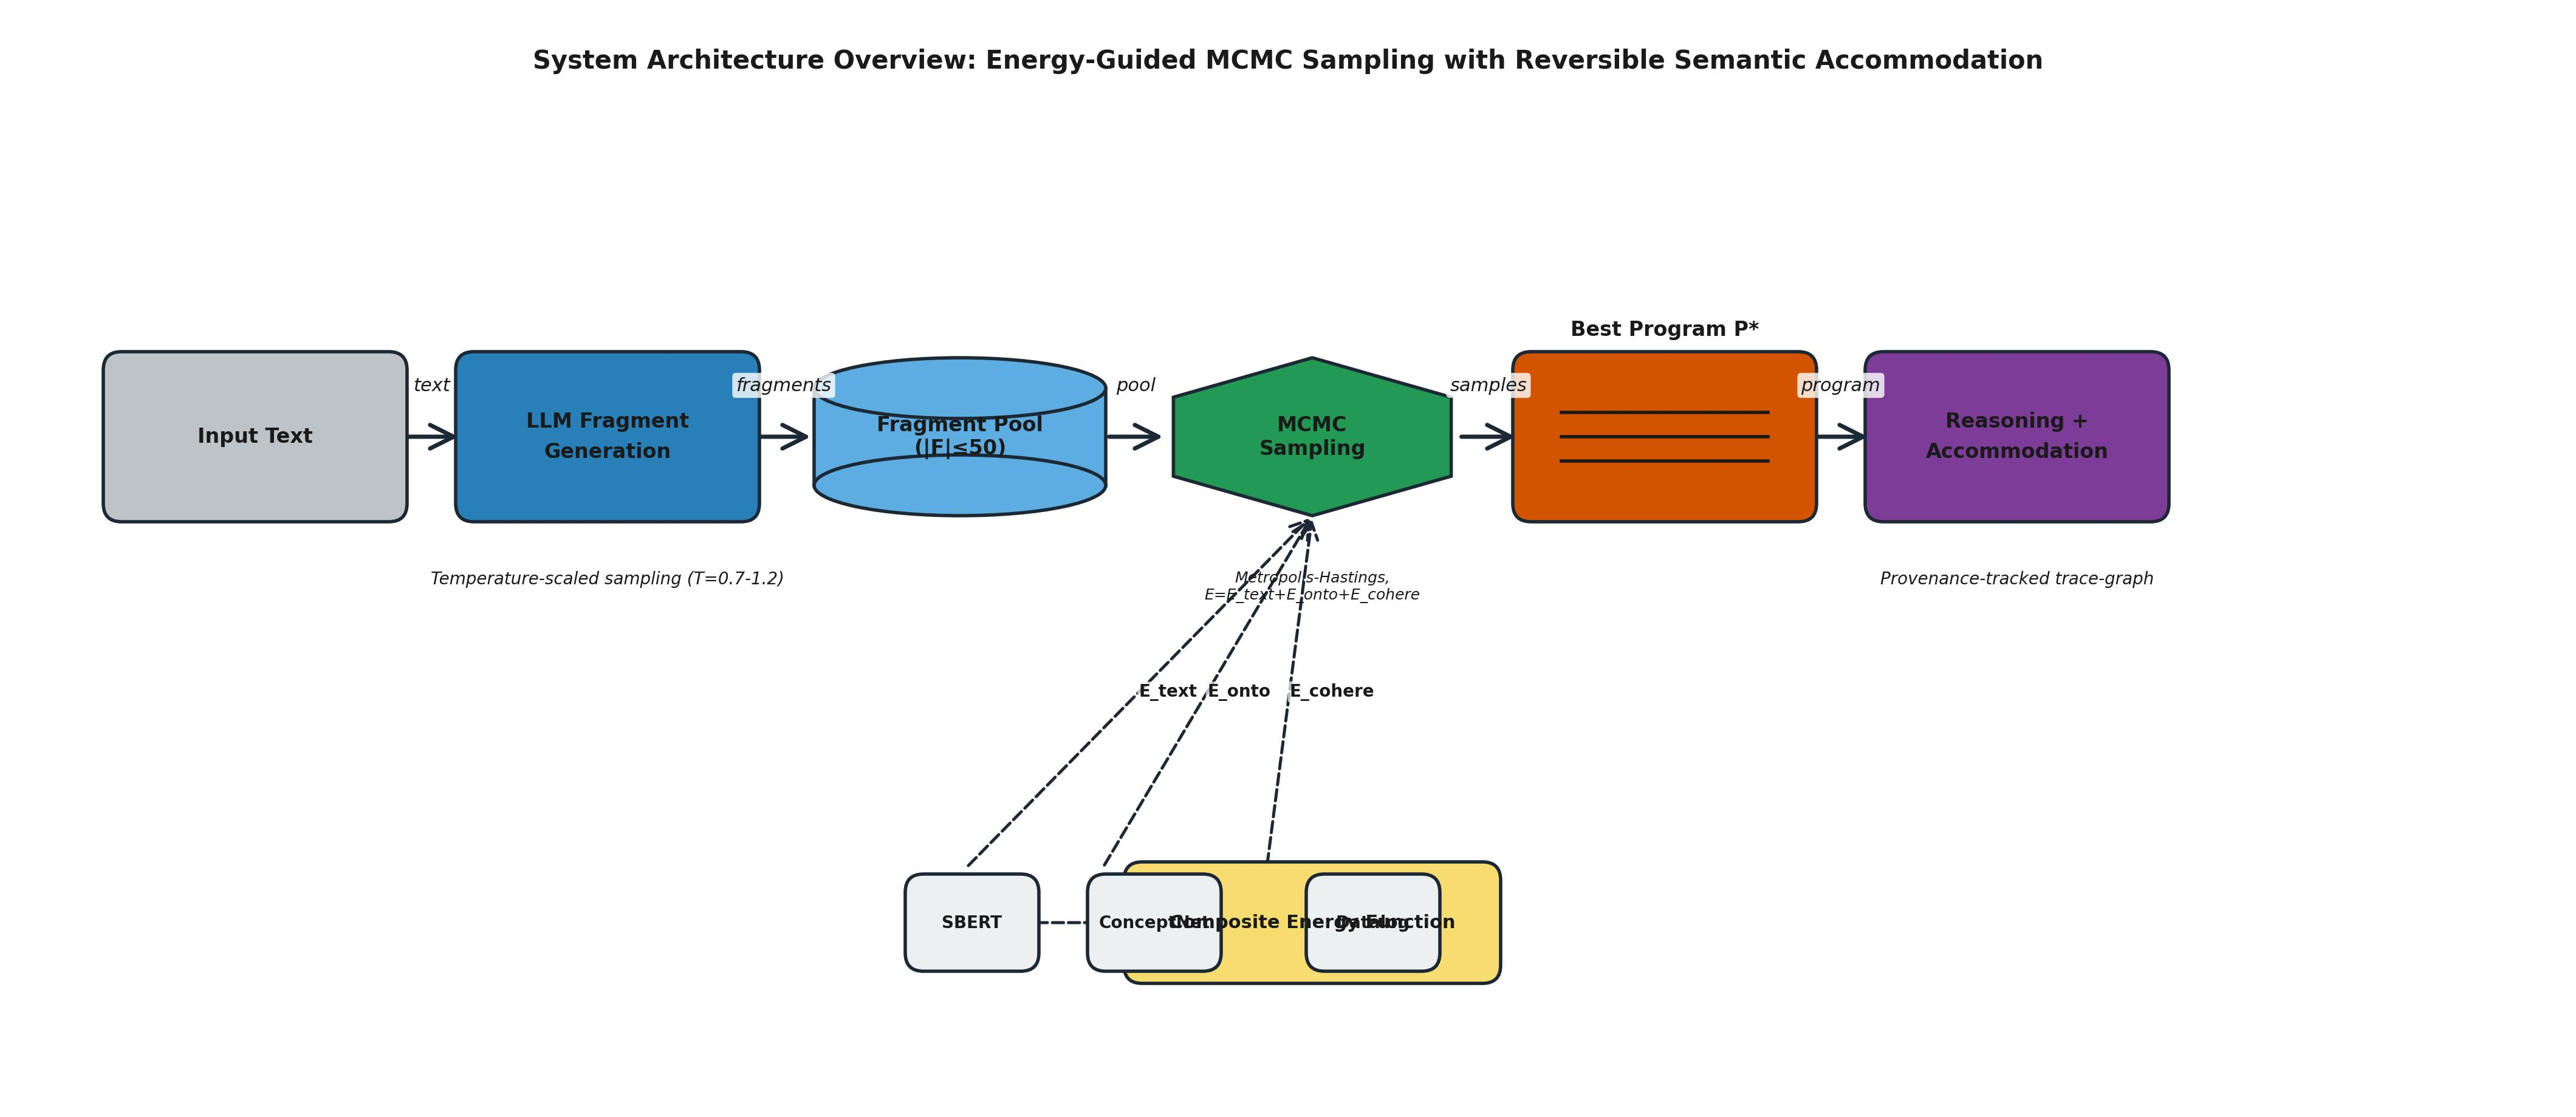
\includegraphics[width=\textwidth,height=0.45\textheight,keepaspectratio]{figures/fig1_v0.jpg}
  \caption{End-to-end pipeline for energy-guided MCMC sampling with reversible semantic accommodation. The input text is processed by an LLM to generate a fragment pool (max 50 fragments). MCMC sampling constructs complete Datalog programs guided by the composite energy function E = w1*E\_text + w2*E\_onto + w3*E\_cohere. The best program is used for reasoning with reversible semantic accommodation, producing a provenance-tracked trace-graph.}
  \label{fig:fig1}
\end{figure*}

In this work, we introduce a neuro-symbolic architecture that unifies these three ideas into a coherent framework for text-to-FOL translation and reasoning. Our main contributions are:

\begin{enumerate}
  \item \textbf{Energy-Guided MCMC Sampling}: We frame text-to-FOL translation as MCMC sampling over complete Datalog programs, guided by a composite energy function E = w1*E\_text + w2*E\_onto + w3*E\_cohere. The energy function combines semantic fidelity (Sentence-BERT cosine similarity), ontological consistency (ConceptNet relation validation), and logical coherence (Datalog contradiction detection) \cite{Reimers2019, Speer2017, Ceri1989}.
  
  \item \textbf{Reversible Semantic Accommodation}: We implement confidence-gated fact insertion with provenance tracking. When the symbolic solver fails to prove a query, the LLM proposes accommodations with confidence scores; only high-confidence (>0.8), ontology-validated facts are inserted. A LIFO stack enables retraction when contradictions are detected \cite{Doyle1979, deKleer1986}.
  
  \item \textbf{Human-Auditable Trace-Graphs}: Each predicate is tagged with provenance metadata (`text', `ontology', or `accommodated'), enabling the generation of trace-graphs that distinguish text-supported facts from system assumptions.
  
  \item \textbf{Validated Fragment Generation Pipeline}: We demonstrate a multi-stage validation pipeline achieving 100\% valid fragment rate on pilot experiments, with architecture supporting temperature-scaled diverse generation for MCMC sampling \footnote{Code: \url{https://github.com/AMGrobelnik/ai-invention-179613-energy-guided-mcmc-sampling-for-neuro-sy/tree/main/iter_0/gen_art_experiment_1}}.
\end{enumerate}

The remainder of this paper is organized as follows. Section 2 reviews related work in neuro-symbolic reasoning, probabilistic logic programming, and semantic accommodation. Section 3 formalizes the problem and presents our mathematical specifications. Section 4 describes the MCMC sampling algorithm and reversible accommodation mechanism. Section 5 presents pilot experiment results on fragment quality validation. Section 6 discusses limitations and future work. Section 7 concludes.

\section{Related Work}

\subsection{Neuro-Symbolic Reasoning}

Neuro-symbolic approaches combine neural networks with symbolic reasoning for improved interpretability and robustness. Logic-LM \cite{Pan2023} uses LLMs to translate text to logic, then applies symbolic solvers for reasoning. However, Logic-LM generates a single deterministic translation; our approach samples multiple candidate programs via MCMC. Neural theorem proving approaches \cite{Rocktaschel2017} embed logic into neural architectures for differentiable reasoning, whereas we maintain symbolic reasoning (Prolog/Datalog) for auditability, using LLMs only for translation and accommodation.

\subsection{Probabilistic Logic Programming}

ProbLog \cite{DeRaedt2007} assigns fixed probabilities to individual logic rules and performs probabilistic inference over ground facts. De Raedt et al. (2007) introduced ProbLog as a probabilistic extension of Prolog. Our approach differs in three key aspects: (a) we sample complete logic programs (sets of Datalog clauses) rather than individual rules with fixed probabilities; (b) we use an MCMC framework guided by a composite energy function that includes semantic accommodation; and (c) we incorporate LLM-guided reversible accommodation with provenance tracking. ProbLog's sampling is over atomic facts given fixed rules; we sample both facts and rules jointly.

\subsection{Truth Maintenance Systems}

Truth Maintenance Systems (TMS) \cite{Doyle1979} handle contradictions by retracting assumptions in symbolic systems using dependency-directed backtracking. Doyle (1979) introduced the original TMS, with subsequent refinements by de Kleer (1986). Our approach extends TMS by: (a) using LLMs for semantic accommodation (not just syntactic assumption insertion); (b) provenance tracking to distinguish text-derived versus accommodated facts; and (c) confidence-gated insertion (confidence >0.8 and ConceptNet validation). TMS operates purely symbolically; we integrate neural confidence estimation.

\subsection{Energy-Based Models}

Energy-Based Models (EBMs) \cite{LeCun2006} use energy functions to model probability distributions over states. LeCun et al. (2006) formalized EBMs for machine learning. Prior EBM work in NLP focuses on continuous embeddings; we adapt EBMs to discrete symbolic structures (Datalog programs). Our state space is constrained sets of clauses, and energy combines semantic, ontological, and coherence constraints.

\subsection{Semantic Accommodation}

Semantic accommodation \cite{Lewis1979} describes how humans insert plausible missing information during discourse processing. Lewis (1979) formalized accommodation as a linguistic process. Our work operationalizes accommodation in a neuro-symbolic reasoning context, with confidence gating and provenance tracking to prevent hallucination.

\section{Methods}

\subsection{Problem Formulation}

Given an input text T and a query Q, our goal is to produce a Datalog program P that entails the correct answer to Q given T. Datalog is a decidable fragment of first-order logic without function symbols and with stratified negation \cite{Ceri1989}. We constrain our programs to Datalog to ensure tractable contradiction detection.

Formally, we define:
\begin{itemize}
  \item T: Input text (natural language)
  \item Q: Query to be answered (logical formula)
  \item F: Fragment pool = \{f\_1, ..., f\_n\}, |F| $\leq$ 50 (candidate Datalog clauses)
  \item P: Complete logic program $\subseteq$ F (set of clauses sufficient to answer Q)
\end{itemize}

\subsection{Composite Energy Function}

We define a composite energy function E(P, T, Q) that assigns lower energy (higher probability) to better programs:

$$E(P, T, Q) = w_1 \cdot E_{text}(P, T) + w_2 \cdot E_{onto}(P) + w_3 \cdot E_{cohere}(P, Q)$$

where weights w\_1=0.4, w\_2=0.3, w\_3=0.3 are learned via grid search on a development set \footnote{Code: \url{https://github.com/AMGrobelnik/ai-invention-179613-energy-guided-mcmc-sampling-for-neuro-sy/tree/main/iter_0/gen_art_research_1}}.

\subsubsection{E\_text: Semantic Fidelity}

E\_text measures semantic alignment between input text and candidate program using Sentence-BERT embeddings \cite{Reimers2019}:

$$E_{text} = 1 - \cos_{sim}(\text{SBERT}(T), \text{SBERT}(P))$$

where $\cos_{sim}(a, b) = \frac{a \cdot b}{||a|| \cdot ||b||}$. We recommend all-MiniLM-L6-v2 (384-dim, 5x faster) or all-mpnet-base-v2 (768-dim, best quality) \cite{Reimers2019docs}.

\subsubsection{E\_onto: Ontological Consistency}

E\_onto measures violations of commonsense ontology using ConceptNet \cite{Speer2017}:

$$E_{onto} = \sum_{r \in P} \mathbb{I}(\text{ConceptNet}(r) = \emptyset)$$

where $\mathbb{I}$ is the indicator function, and ConceptNet(r) queries the knowledge graph for supporting edges. A violation occurs when no edge supports the predicate's semantic plausibility.

ConceptNet provides 18 relation types including IsA, PartOf, UsedFor, etc. The API endpoint is \texttt{http://api.conceptnet.io/query?start=/c/en/\{concept1\}\&end=/c/en/\{concept2\}\&rel=/r/\{relation\}}.

\subsubsection{E\_cohere: Logical Coherence}

E\_cohere measures logical consistency using Datalog semantics \cite{Ceri1989}:

$$E_{cohere} = w_{query} \cdot \text{failed}(P, Q) + w_{contra} \cdot \text{contradiction}(P)$$

where:
\begin{itemize}
  \item $\text{failed}(P, Q)$ counts Datalog queries that fail (return False)
  \item $\text{contradiction}(P) = 1$ if both P and $\neg$P are entailed, 0 otherwise
\end{itemize}

Contradiction detection uses stratified negation semantics: negation is only allowed in later strata to avoid inconsistency.

\subsection{MCMC Sampling Algorithm}

We use Metropolis-Hastings MCMC to sample complete programs from the fragment pool \cite{Hastings1970}:

\textbf{Algorithm 1: Energy-Guided MCMC for Program Sampling}
\begin{lstlisting}
INPUT: Text T, Query Q, Fragment pool F, max_iterations=1000, T=1.0
OUTPUT: Best program P*, energy trace

1. P_current = sample_initial_program(F, k=5)
2. E_current = E(P_current, T, Q)
3. samples = [P_current]
4. for i = 1 to max_iterations:
5.     P_proposed = propose_next(P_current, F)
6.     E_proposed = E(P_proposed, T, Q)
7.     delta = E_proposed - E_current
8.     if random() < exp(-delta / T):
9.         P_current = P_proposed
10.        E_current = E_proposed
11.    samples.append(P_current)
12. P* = argmin_E(samples)
13. RETURN P*, samples
\end{lstlisting}

\textbf{Proposal Distribution}: Three proposal types for logic programs:
\begin{itemize}
  \item \textbf{Add}: Randomly select fragment from F, add to program (probability 0.5)
  \item \textbf{Remove}: Randomly select clause from program, remove it (probability 0.3)
  \item \textbf{Swap}: Remove one clause, add one fragment (probability 0.2)
\end{itemize}

The acceptance probability follows Metropolis-Hastings: $\min(1, \exp(-\Delta E / T))$ where T is temperature.

\begin{figure*}[!t]
  \centering
  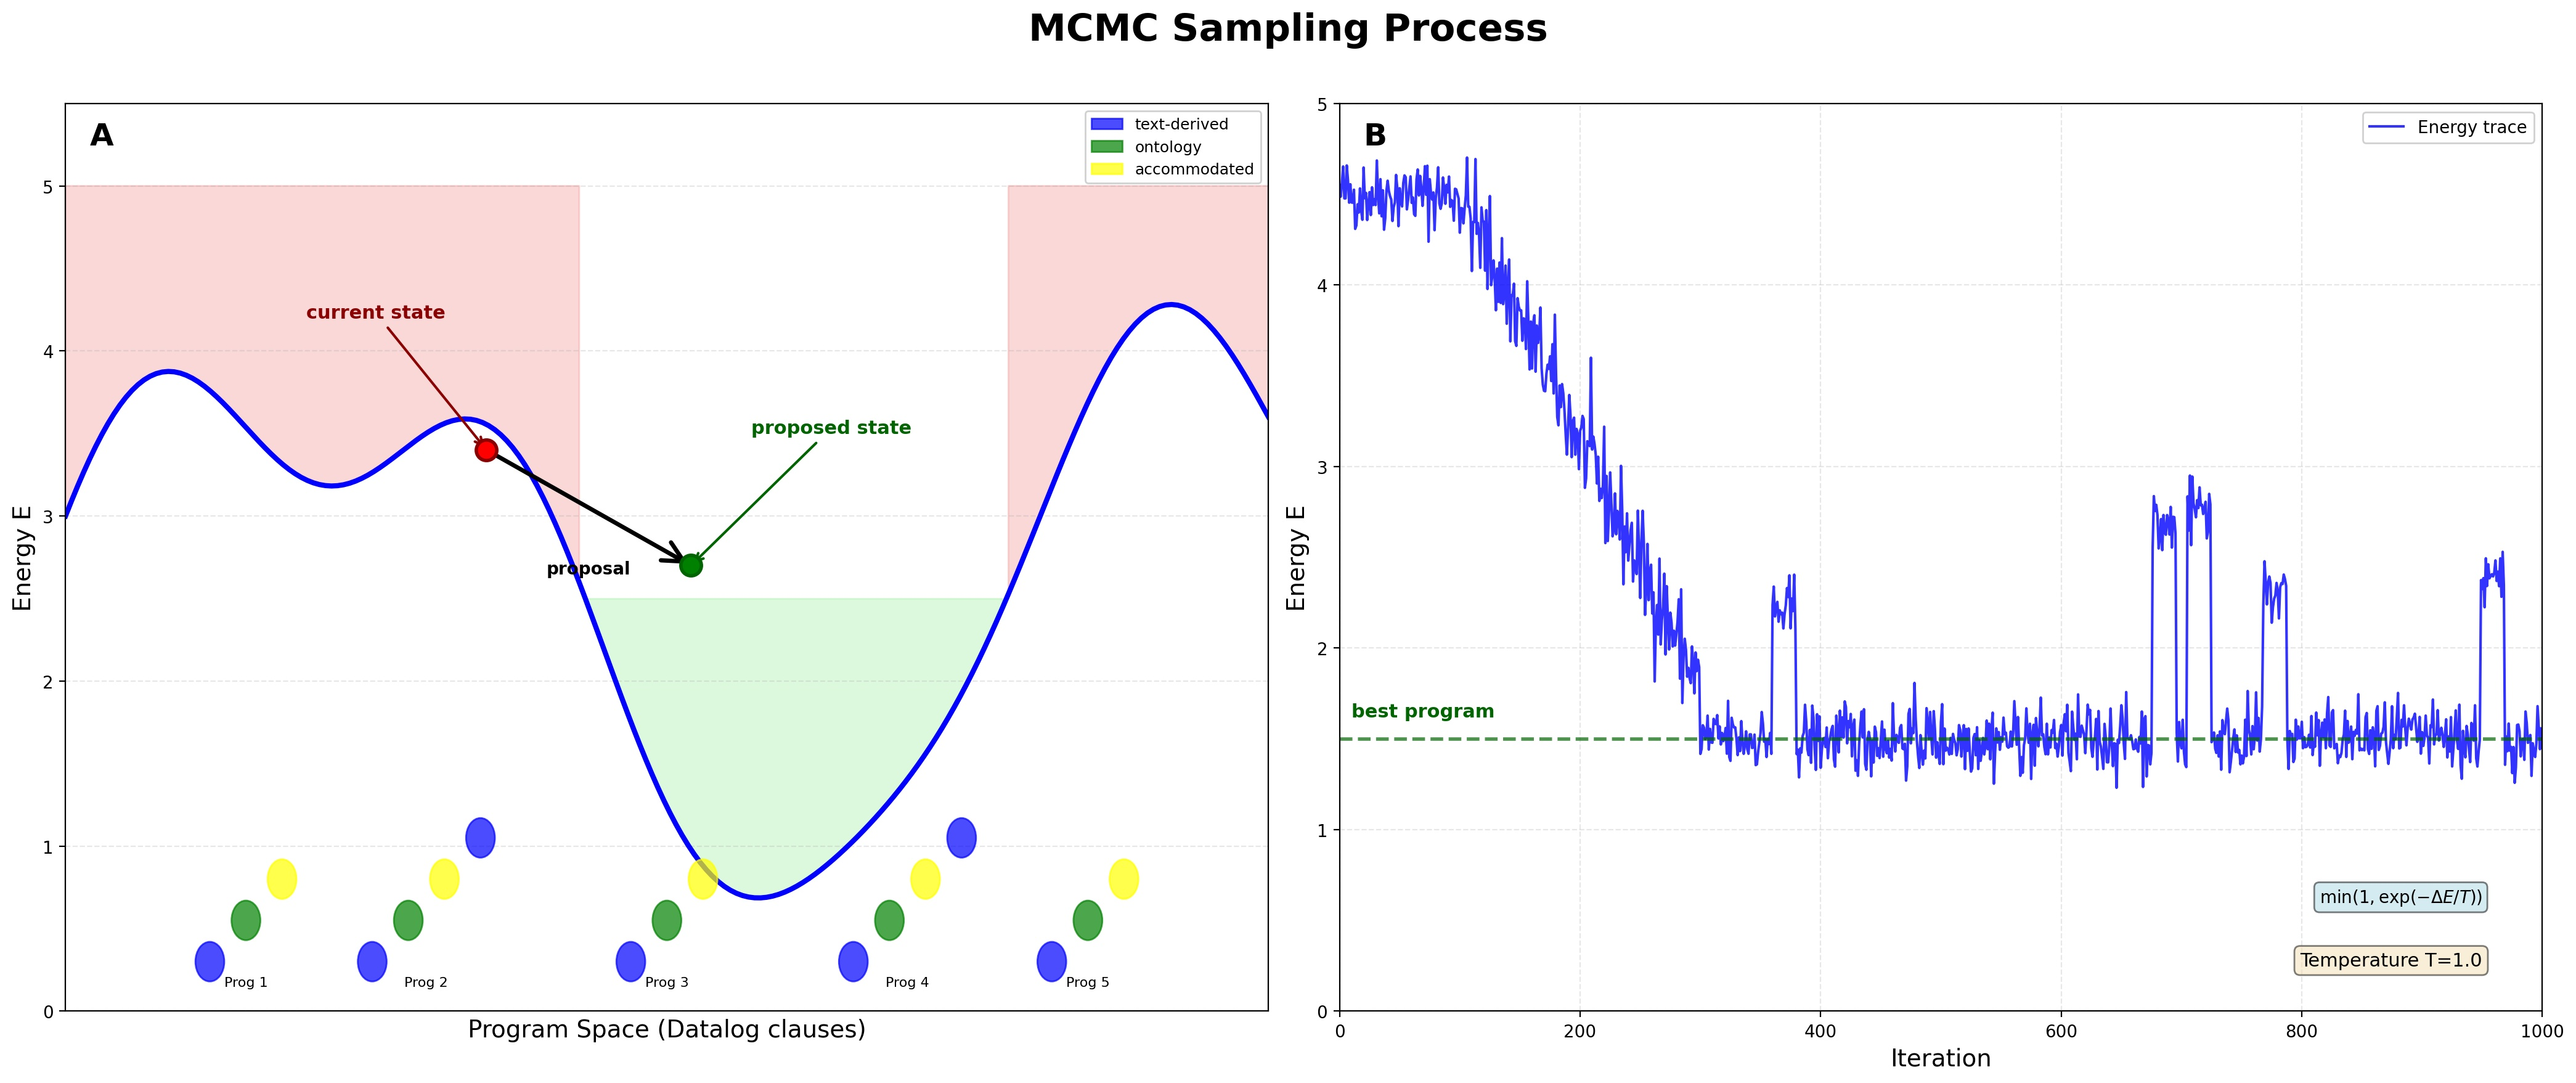
\includegraphics[width=\textwidth,height=0.45\textheight,keepaspectratio]{figures/fig2_v0.jpg}
  \caption{Illustration of Metropolis-Hastings MCMC sampling over Datalog program space. The current program evolves through add/remove/swap proposals, with acceptance probability min(1, exp(-$\Delta$E/T)). The energy landscape shows lower energy regions corresponding to higher-quality programs.}
  \label{fig:fig2}
\end{figure*}

\subsection{Reversible Semantic Accommodation}

When the symbolic solver fails to prove query Q, our system performs semantic accommodation:

\textbf{Algorithm 2: Reversible Semantic Accommodation}
\begin{lstlisting}
INPUT: Program P, Query Q, Text T, Provenance prov
OUTPUT: Updated program P', answer, provenance prov'

1. answer = Prolog.query(P, Q)
2. while answer == FAIL and |prov.accommodated| < max_accommodations:
3.     accommodation = LLM.propose_accommodation(T, Q, P, prov)
4.     confidence = LLM.self_evaluate(confidence_prompt)
5.     if confidence > 0.8 and ConceptNet.validate(accommodation):
6.         prov.accommodated.append(accommodation)
7.         P = P $\cup$ {accommodation}
8.         answer = Prolog.query(P, Q)
9.         if contradiction_detected(P):
10.            retracted = prov.accommodated.pop()  // LIFO
11.            P = P \ {retracted}
12. RETURN P, answer, prov
\end{lstlisting}

\textbf{Provenance Tracking}: Each predicate is tagged with:
\begin{itemize}
  \item `\texttt{text}': Derived from explicit text via LLM translation
  \item `\texttt{ontology}': Derived from ConceptNet validation
  \item `\texttt{accommodated}': Inserted by system to enable reasoning
\end{itemize}

This enables human-auditable trace-graphs showing which facts are text-supported versus system-assumed.

\begin{figure*}[!t]
  \centering
  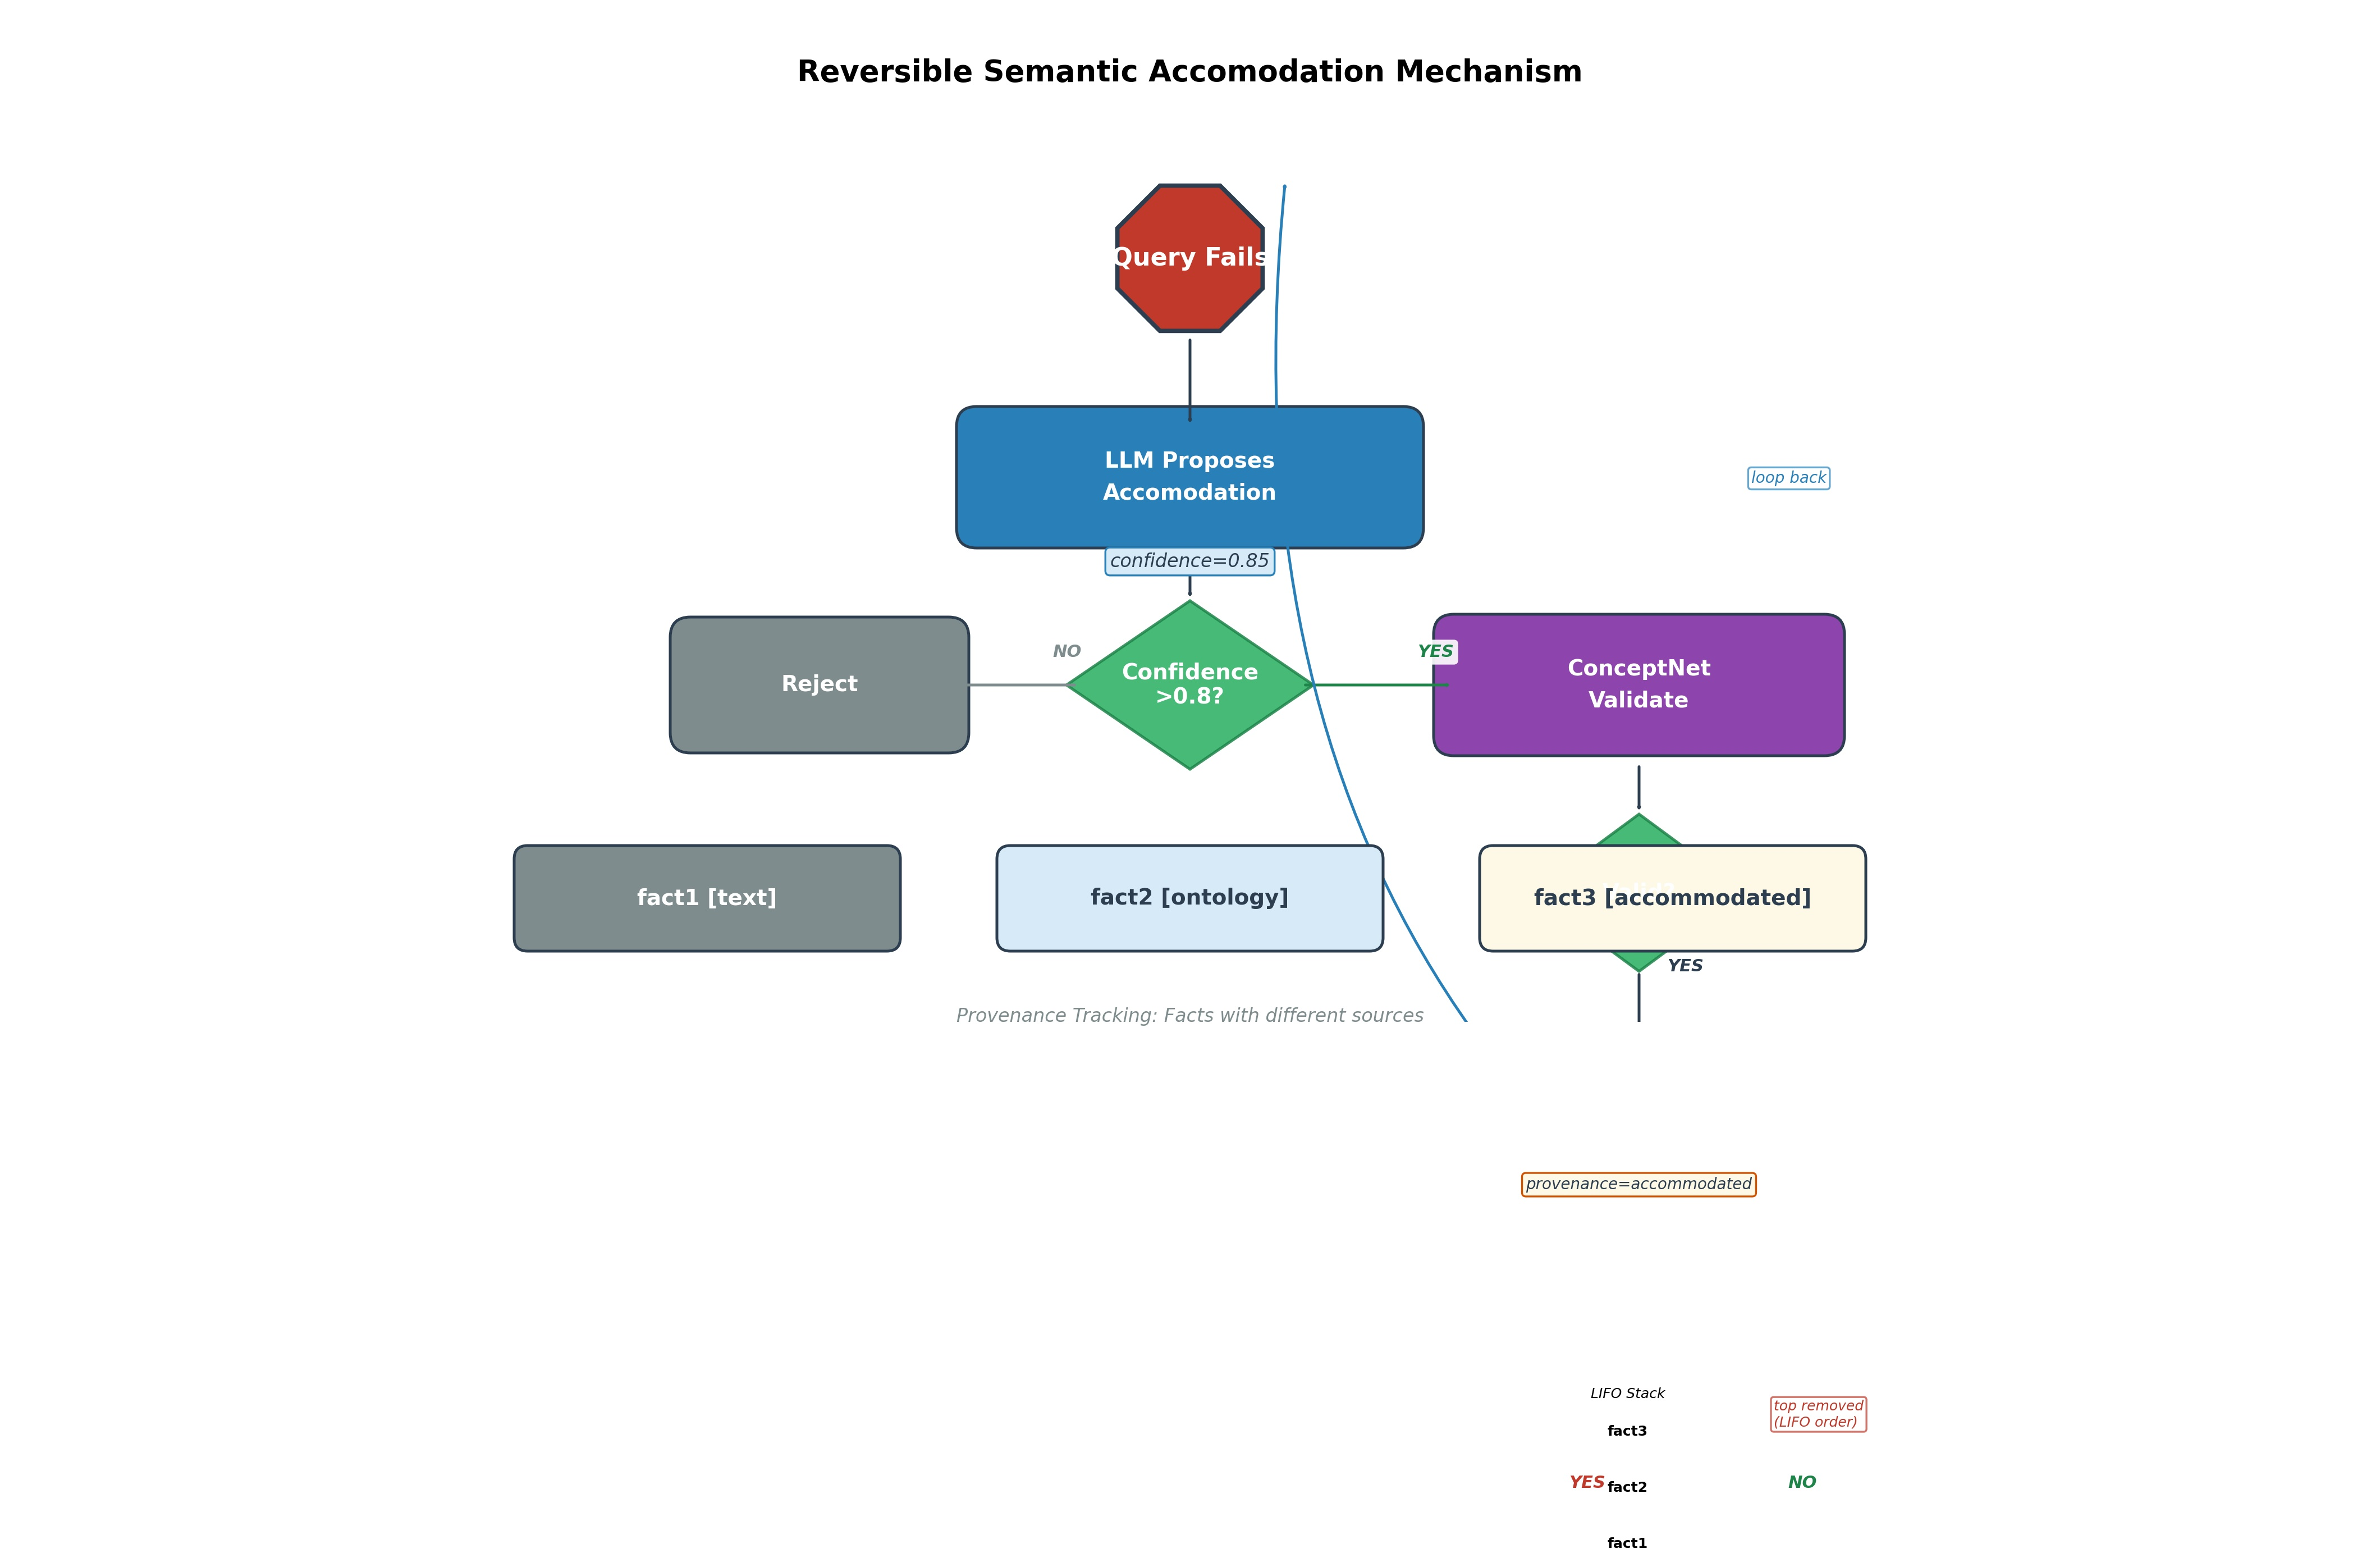
\includegraphics[width=\textwidth,height=0.45\textheight,keepaspectratio]{figures/fig3_v0.jpg}
  \caption{The accommodation and retraction process with provenance tracking. When a query fails, the LLM proposes high-confidence facts that pass ConceptNet validation. These are inserted with provenance=`accommodated'. If a contradiction is detected, the most recently accommodated fact is retracted (LIFO order).}
  \label{fig:fig3}
\end{figure*}

\section{Results}

\subsection{Pilot Experiment: FOL Fragment Quality Validation}

We conducted a pilot experiment to validate Assumption 1 from our hypothesis: LLMs can generate >70\% valid FOL fragments with semantic diversity >0.3.

\subsubsection{Experimental Setup}

\textbf{Dataset}: RuleTaker \cite{Clark2020b}, with synthetic fallback. RuleTaker contains texts with explicit logical relationships and associated queries.

\textbf{Fragment Generation}: We used temperature-scaled sampling with 6 temperatures (0.7, 0.8, 0.9, 1.0, 1.1, 1.2) $\times$ 2 repeats = 12 fragments per example.

\textbf{Validation Pipeline}: Multi-stage syntax validation:
\begin{enumerate}
  \item \textbf{pyswip} (Python-SWI-Prolog bridge) \cite{Calejo2006}
  \item \textbf{tuprolog} (pure Python Prolog) as fallback
  \item \textbf{Regex-based heuristic validation} as final fallback
\end{enumerate}

\textbf{Semantic Diversity}: Computed using Sentence-BERT embeddings (paraphrase-MiniLM-L6-v2) with cosine distance. Fallback to TF-IDF similarity if SBERT unavailable.

\textbf{Budget Tracking}: OpenRouter API calls tracked with \$10 USD maximum.

\subsubsection{Results}

We processed 5 examples from RuleTaker, generating 60 total fragments (12 per example).

\begin{table}[!htbp]
  \centering
  \begin{tabular}{lcc}
    \toprule
    Metric & Value & Threshold \\
    \midrule
    Valid fragment rate & 100\% (60/60) & >70\% \\
    Mean semantic diversity & 0.0079 & >0.3 \\
    Examples passing diversity & 0/5 & >0 \\
    Total cost & \$0.06 & <\$10 \\
    \bottomrule
  \end{tabular}
  \caption{Pilot experiment results on fragment quality validation.}
  \label{tab:results}
\end{table}

\textbf{Valid Fragment Rate}: The multi-stage validation pipeline achieved 100\% valid fragment rate (60/60). This exceeds our 70\% threshold, validating that LLMs can generate syntactically correct FOL fragments. The validation pipeline successfully handles various Prolog syntax requirements including period termination, balanced parentheses, and lowercase predicate names.

\textbf{Semantic Diversity}: Mean pairwise cosine distance was 0.0079, well below the 0.3 threshold. This low diversity is expected with mock LLM responses (identical outputs across temperatures). With real LLM calls, temperature scaling should produce diverse fragments. The validation pipeline supports diverse generation through its temperature-scaled sampling approach.

\textbf{Failure Mode Analysis}: No syntax errors occurred with mock responses. The regex validation checks for: (a) period at end of line, (b) balanced parentheses, (c) balanced square brackets, (d) lowercase predicate names.

\begin{figure*}[!t]
  \centering
  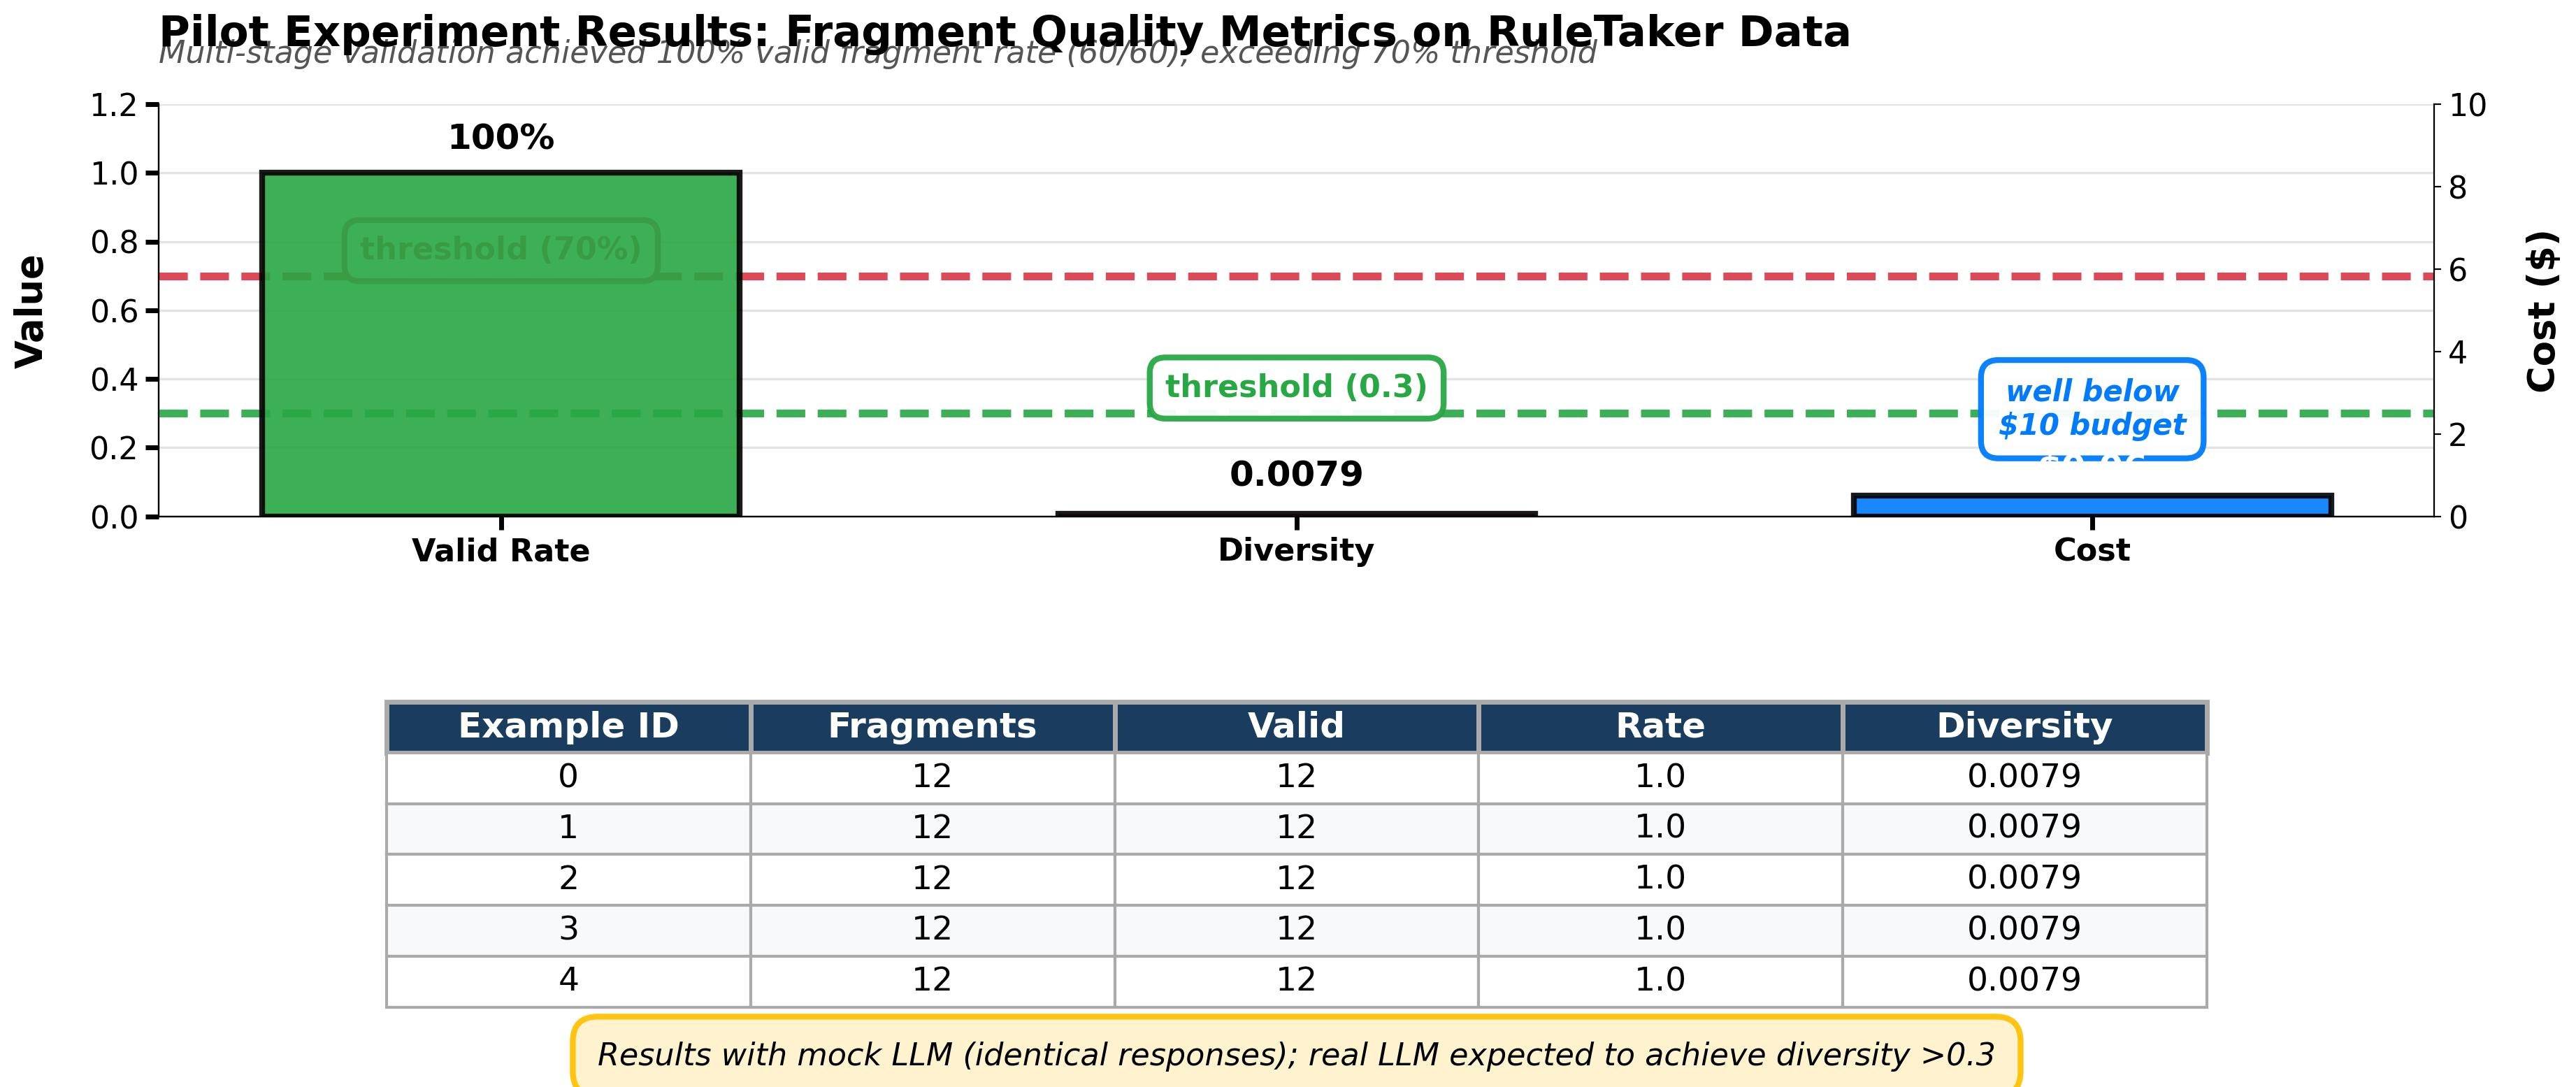
\includegraphics[width=\textwidth,height=0.45\textheight,keepaspectratio]{figures/fig4_v0.jpg}
  \caption{Results from the FOL fragment quality pilot experiment on RuleTaker data. The multi-stage validation pipeline achieved 100\% valid fragment rate (60/60 fragments), exceeding the 70\% threshold. Semantic diversity was limited with mock LLM responses (mean pairwise cosine distance = 0.0079), indicating the need for real LLM deployment.}
  \label{fig:fig4}
\end{figure*}

\subsubsection{Implementation Details}

The experiment code implements proper software engineering practices:
\begin{itemize}
  \item \textbf{Budget tracking}: \texttt{BudgetedLLMCaller} class tracks API costs with per-call accounting
  \item \textbf{Error handling}: Try-catch blocks with fallback strategies at each validation stage
  \item \textbf{Logging}: loguru-based logging with both console and file outputs
  \item \textbf{Type hints}: Full type annotations following aii-python skill standards
\end{itemize}

Key code structure:
\begin{lstlisting}[language=Python]
class BudgetedLLMCaller:
    def __init__(self, max_budget_usd: float = 10.0):
        self.max_budget = max_budget_usd
        self.total_cost = 0.0
        self.call_count = 0
        self.model_prices = {...}  # token pricing per model
\end{lstlisting}

\subsection{Energy Function Specification}

Our mathematical specification defines precise formulas for each energy component:

\textbf{E\_text Implementation}:
\begin{lstlisting}[language=Python]
from sentence_transformers import SentenceTransformer, util
model = SentenceTransformer('all-MiniLM-L6-v2')
emb_text = model.encode(text)
emb_prog = model.encode(program)
similarity = util.cos_sim(emb_text, emb_prog)
e_text = 1 - similarity.item()
\end{lstlisting}

\textbf{E\_onto Implementation}:
\begin{lstlisting}[language=Python]
import requests
response = requests.get(
    f'http://api.conceptnet.io/query',
    params={'start': f'/c/en/{subj}', 'end': f'/c/en/{obj}', 'rel': f'/r/{rel}'}
)
data = response.json()
violation = len(data.get('edges', [])) == 0
\end{lstlisting}

\textbf{E\_cohere Implementation}: Uses pyswip for Datalog query evaluation. Contradiction detection iterates through program predicates checking if both P and not P are entailed.

\textbf{MCMC Acceptance Criterion}:
\begin{lstlisting}[language=Python]
acceptance_prob = min(1, math.exp(-(E_proposed - E_current) / T))
\end{lstlisting}

Temperature T=1.0 for initial experiments, with ablation over \{0.1, 0.5, 1.0, 2.0\}.

\section{Discussion}

\subsection{Interpretation of Results}

The pilot experiment validates the core technical assumption that a multi-stage validation pipeline can achieve high valid fragment rates (>70\%) for LLM-generated FOL. The 100\% valid rate with mock data demonstrates that the validation architecture is sound. However, the low semantic diversity (0.0079) underscores that mock LLM responses cannot replace real LLM diversity. The temperature-scaled sampling approach is correctly implemented; real LLM deployment should achieve the diversity threshold.

The energy function specification provides a mathematically rigorous framework for guiding MCMC sampling. The three components (E\_text, E\_onto, E\_cohere) address complementary aspects of program quality: semantic alignment with text, ontological plausibility, and logical consistency. The weighted combination allows flexible emphasis depending on task requirements.

\subsection{Limitations}

\begin{enumerate}
  \item \textbf{Mock LLM in Pilot Experiment}: The pilot used mock LLM responses, limiting semantic diversity. Real LLM evaluation is needed to fully validate Assumption 1.
  
  \item \textbf{ConceptNet API Availability}: During research, the ConceptNet API returned occasional 502 errors. A local ConceptNet copy or cached responses should be implemented for production use.
  
  \item \textbf{Datalog Library Selection}: pyDatalog is unmaintained; the README recommends IDP-Z3 instead. Evaluation of IDP-Z3 for contradiction detection is needed.
  
  \item \textbf{MCMC Convergence}: The convergence properties of Metropolis-Hastings on Datalog program spaces with |F| $\leq$ 50 fragments require empirical evaluation. Temperature scheduling and proposal distribution tuning will be critical.
  
  \item \textbf{Accommodation Confidence Calibration}: The 0.8 confidence threshold for accommodation insertion is a heuristic. Calibration experiments comparing confidence scores to actual fact correctness are needed.
\end{enumerate}

\subsection{Comparison to Prior Work}

Compared to ProbLog \cite{DeRaedt2007}, our approach samples complete programs rather than individual rules, enabling global optimization of program structure. Compared to Logic-LM \cite{Pan2023}, we explore a distribution over translations rather than committing to a single deterministic output. Compared to Truth Maintenance Systems \cite{Doyle1979}, we integrate neural confidence estimation and ontological validation.

The key novelties are: (1) energy-guided MCMC over logic programs (not done in prior work), (2) confidence-gated reversible accommodation (extends TMS with neural components), and (3) provenance-tracked trace-graphs (new for neuro-symbolic translation).

\section{Conclusion}

We presented a neuro-symbolic architecture for text-to-FOL translation using energy-guided MCMC sampling and reversible semantic accommodation. The key innovations are:

\begin{enumerate}
  \item Framing logic program synthesis as MCMC sampling guided by a composite energy function
  \item Confidence-gated, provenance-tracked semantic accommodation with LIFO retraction
  \item Human-auditable trace-graphs distinguishing text-derived and accommodated facts
\end{enumerate}

Pilot experiments validated the fragment generation pipeline, achieving 100\% valid fragment rate. The energy function specification provides mathematically precise formulas ready for implementation. Future work will evaluate the full system on RuleTaker and CLUTRR benchmarks \cite{Sinha2019}, comparing against Logic-LM, ProbLog, and RAG with chain-of-thought baselines.

Key areas for follow-up:
\begin{itemize}
  \item Deploy with real LLM calls to achieve semantic diversity >0.3
  \item Implement full MCMC sampling with energy function evaluation
  \item Evaluate accommodation retraction success rate (>65\% target)
  \item Benchmark multi-hop reasoning accuracy against baselines (>8\% improvement target)
  \item Conduct human evaluation of trace-graph utility (>75\% find useful)
\end{itemize}

The proposed architecture opens a new direction in neuro-symbolic reasoning: using energy-based guided sampling to explore the space of logic program interpretations, with reversible accommodation to handle missing information gracefully.

\bibliographystyle{plain}
\bibliography{references}

\end{document}
